\documentclass{hessothesis}

\ThesisTitle{APDL : Acquire Process Description Language}
\Author{Sylvain Julmy}
\Supervisor{Pierre-André Mudry}
\SupervisorResearchUnit{Institut Systèmes Industriels}
\ExternalExpert{??}
\ExternalExpertResearchUnit{??}
\Place{Lausanne}
\Date{\today}
\AuthorEmail{sylvain.julmy@gmail.com}
\Orientation{Information and Communication Technologies (ICT)}

\bibliography{bibliography.bib}

\newacronym{IoT}{IoT}{Internet of Things}
\newacronym{DSL}{DSL}{Domain specific language}
\newacronym{VDSML}{VDSML}{Visual Domain Specific Modeling Language}
\newacronym{APDL}{APDL}{Acquire and Process Description Language}

%%% Local Variables:
%%% mode: latex
%%% TeX-master: "thesis"
%%% End:


\begin{document}

\maketitle
\makeinfopage

\tableofcontents

\newChapter{Introduction}{cha:introduction}

The \gls{IoT} is one of the most prolific domains in computer science
nowadays. There are connected objects everywhere and the amount of data that we
receive from them is growing day after day. Everybody wants to measure some
environment variables using a simple and cheap device like an Arduino or a
Raspberry Pi.

On another hand, people who want to use those devices are often not familiar
with the hardware and/or the software parts of an IoT project. For example, a
chemistry engineer could be interested to measure some values in the air, but he
is absolutely not in the IoT domain.

\section{Context}
\label{sec:intro-context}

Imagine an electrical engineer who needs to create a system which is able to
recover data from multiple sensors, like external temperature and barometric
pressure. With that data, the engineer needs to compute a new pressure value
with the temperature and compare it to the one given by the barometric pressure
sensor using graph plot.

The problem for this electrical engineer is the software part. He doesn't know how
to send data through the network, recover them and store them into a database
for a future plot. On another hand, a software engineer would not know the hardware part.

IoT programming is at some point a merge of some specific domains like Software,
Hardware, Telecommunication and Design. The figure \ref{fig:basic_archi} illustrates
this concept of multi-domain project. Are involved in this concept:

\begin{itemize}
\item Hardware.
\item Software.
\item Design.
\item Telecommunication.
\end{itemize}

\begin{figure}[H]
  \centering
  \fbox{
    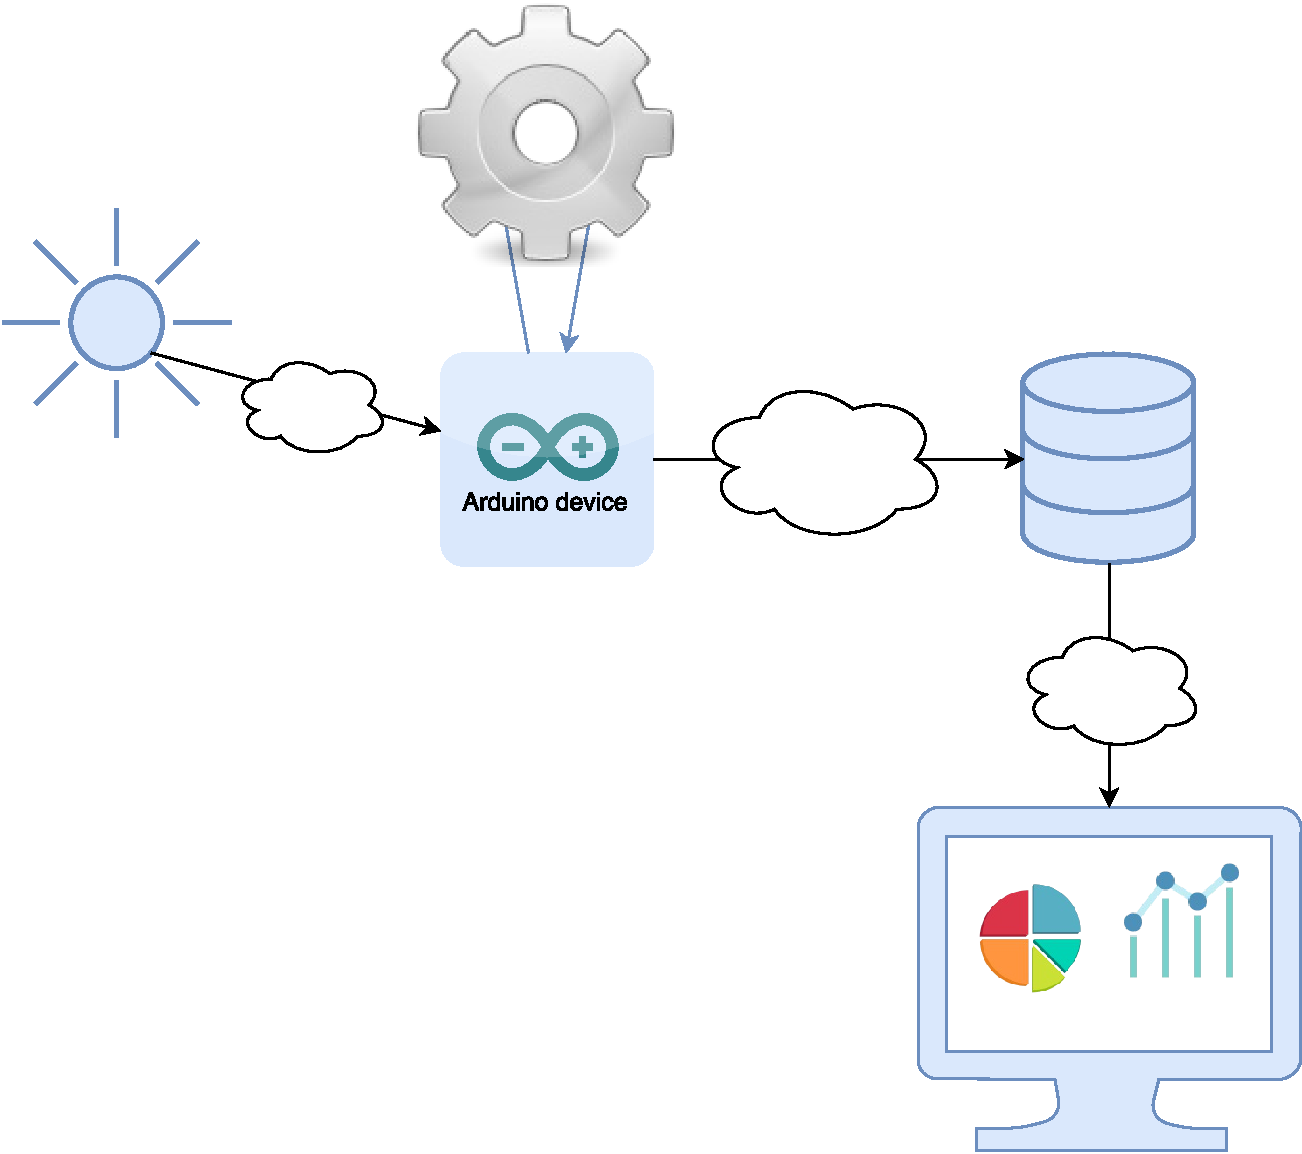
\includegraphics[width=0.4\textwidth]{img/basic_archi}
    }
  \caption[Basic APDL architecture example]{ Visualisation of the involved domains
in the APDL ecosystem : hardware, software, design and
telecommunication. And sometimes, a person doesn't know any part of this.}
  \label{fig:basic_archi}
\end{figure}

\section{Problem Statement}
\label{sec:intro-problem-statement}

According to the previous example we could say that not everybody could develop
a project like this from scratch. Maybe some people have the whole knowledge to
do this by themselves but not a lambda person.

The major issue with such project is the people diversity. Bringing together people from various
professions creates several difficulties : team management, various programming knowledge, different
project's perception, and many more.

\section{Solution Statement}
\label{sec:intro-solution-statement}

The \gls{APDL} ecosystem goal is to
provide a simple way to describe such a pipeline. From the sampling of the data
from a sensor and its transformation to the display of the result of charts through
storing them into a database or send them to a specific server.

\section{Outline of this thesis}
\label{sec:intro-roadmap}

We have set ourselves the challenge of providing a simple way to design specific
\gls{IoT} projects. Before setting out to tackle it, we firstly look at the state
of the art in \gls{DSL} development and \gls{IoT} challenges. Some work has
been done in the field of Domain specific frameworks and languages for \gls{IoT}.

The main technical chapters includes chapter~\ref{chap:dsl_design},
\ref{chap:dsl_implementation}, \ref{chap:dsl_validation}. In
chapter~\ref{chap:dsl_design}, we present the design of the \gls{APDL}
\gls{DSL}. We set out the domain of interest and explore the development process
of the language. Chapter \ref{chap:dsl_implementation} presents the
implementation of the designed language and illustrates the compilation process
used by \gls{APDL}. In chapter \ref{chap:dsl_validation} we present the
validation of the implemented compiler and the generated output based on a set
of APDL programs designed for this purpose. We also mention a testing
technique called property-based testing which has simplified the parser tests.
Finally, in chapter~\ref{chap:apdl_ecosystem}, we present the work done about
the APDL ecosystem and its utilisation through an example realised from scratch.

%%% Local Variables:
%%% mode: latex
%%% TeX-master: "../thesis"
%%% End:


\part{Background}

\newChapter{Domain specific language}
\label{cha:a-dsl}

\section{Introduction}
\label{sec:dsl_intro}

A \gls{DSL} is a programming language whose goal is
to provide a way to solve specific domain problems. For example, Matlab is a
domain specific language created to simplify matrix calculus.

What we call ``domain'' is a set of problem related together in the same scope.
For Matlab, those domains could be a matrix multiplication or the resolution of an
equation system. Those two operations are related to numerical mathematics and
that is the ``domain'' of Matlab.

This chapter introduces and discuss the question : ``Why use a DSL ?'' by
explaining the advantages that a \gls{DSL} could bring for domain-oriented
problems. Then we present the difference between an internal and an external DSL
and the advantages and disadvantages for both of them. Finally, we introduce the
implementation of a \gls{DSL} using the Scala programming language and why Scala
is a great tool for the development of \gls{DSL}.

\section{Why use a DSL ?}
\label{sec:why-use-dsl}

\gls{DSL} exist since the beginning of computing, according to
\cite{VanDeursen2000}, COBOL, Lisp and Fortran have been
created for solving problems in a specific area like business processing, numeric
computations or symbolic processing. With time, language has become more and
more generalist but \gls{DSL} has always been created to simplify some domain
specific problems.

Using a DSL instead of a programming language brings advantages as well as
disadvantages.

\textbf{Advantages:}
\begin{itemize}
\item A high potential of usability and reliability according to
  \cite{Tolvanen2010}.
\item A great learning curve because a DSL is, in general, easier to learn than a
  general programming language \cite{Mernik2005}.
\item An expert of the DSL could modify the application even without knowing how
  to program.
\end{itemize}

\textbf{Disadvantages \cite{VanDeursen2000}:}
\begin{itemize}
\item The cost to develop a DSL : production, user training and
  maintenance.
\item A non-expert user may find hard to modify an existing program.
\item In general, DSL are less efficient than general programming language,
  because programming languages own some very good compiler with a lot of
  optimisations.
\item The need to learn a new language, even if it's a simple one.
\item A DSL don't have any tool support (other than a compiler of course) \cite{Mernik2005}.
\end{itemize}

\section{Internal and External Domain specific language}
\label{sec:internal_and_external_dsl}

It exists two types of \gls{DSL} : internal \gls{DSL}, also call \gls{DSEL} and
external DSL. Understanding the difference, advantages and disadvantages of each
of those is crucial in order to create an appropriate solution to the domain
specific problems.

The main difference between this two concept appears at the compilation time,
the figure \ref{fig:internal_dsl_compilation} shows the compilation of an
internal DSL. The input and the output of the compiler are in the same language.
Then, the figure \ref{fig:external_dsl_compilation} shows the compilation of an
external DSL. This time, we compile the code into another language, called the host language.

\begin{figure}[ht]
  \centering
  \fbox{
    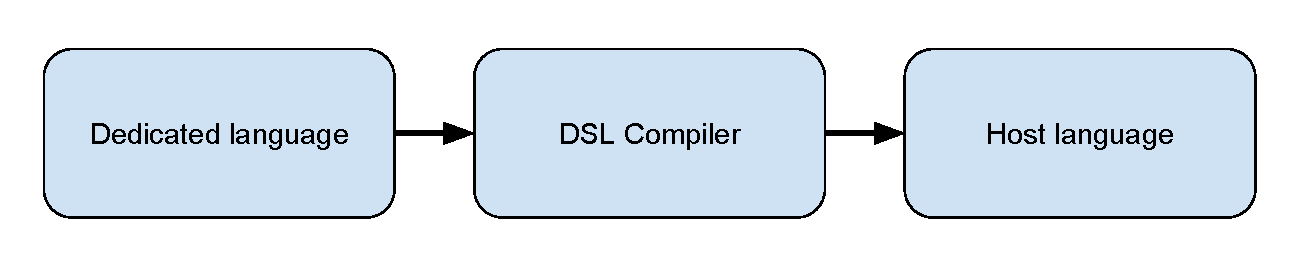
\includegraphics[width=0.8\textwidth]{img/internal_dsl_compilation}
  }
  \caption[Compilation process of an internal \gls{DSL}]{Compilation process of
    an internal Domain specific language. The input and output languages are the
    same. In general, we could see the input language as a library (with or
    without syntactic sugar) for more general programming language.}
  \label{fig:internal_dsl_compilation}
\end{figure}

\begin{figure}[ht]
  \centering
  \fbox{
    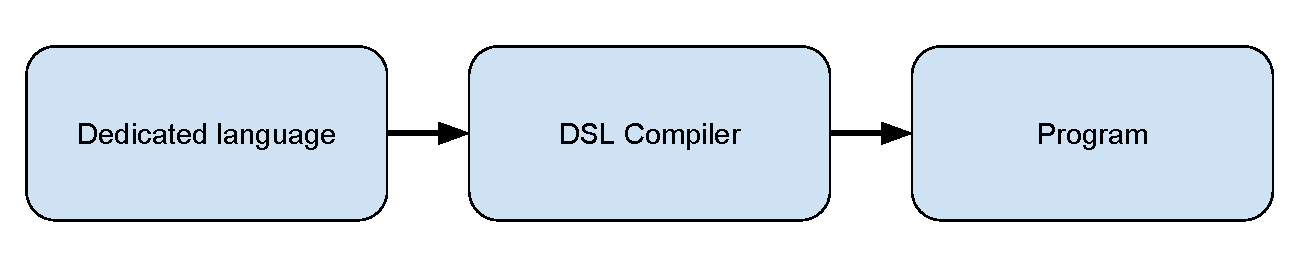
\includegraphics[width=0.8\textwidth]{img/external_dsl_compilation}
   }
  \caption[Compilation process of an external \gls{DSL}]{Compilation process of
    an external Domain specific language. The input and output languages aren't
    the same. This process is closer to a compiler for general language.}
  \label{fig:external_dsl_compilation}
\end{figure}

\subsection{Internal Domain Specific Language}
\label{sec:internal_dsl}

As shown in the figure \ref{fig:internal_dsl_compilation}, the dedicated language
and the output language are the same. Internal \gls{DSL} could be separate into
two categories : \gls{DEDSL} and \gls{SEDSL}.

Conceptually, a \gls{SEDSL} captures the semantic notions of the data's domain in
various data types and manipulate those data in a fixed way. Alternately, a
\gls{DEDSL} goes beyond the captures of semantic notions by capturing the
operations themselves. As an example for understanding those two concepts we look
at listing \ref{lst:deep_vs_shallow_source}. It's a small imaginary DSL used for
temperature manipulation between Kelvin and Celsius. We compute the sum
of three temperatures, and we want to print it in Celsius.

\begin{listing}[ht]
\centering
\begin{scalacode}
val t1 = Celsius(100)
val t2 = Celsius(50)
val t3 = Kelvin(30)
val t4 = t1 + t2 + t3
println(t4 in Celsius)
\end{scalacode}
\caption[Usage of the simple Temperature \gls{DSL}]{Example of the simple
Temperature \gls{DSL}. We simply want to compute the sum of three temperatures,
in Celsius and Kelvin, and finally want to print the result.}
\label{lst:deep_vs_shallow_source}
\end{listing}

Now we are going to compare the simple implementation of this \gls{DSL} for
both \gls{DEDSL} and \gls{SEDSL}. The implementation of the \gls{SEDSL} is
shown in listing \ref{lst:shallow_temp_scala} and for the \gls{DEDSL} in
listing \ref{lst:deep_temp_scala}.

\begin{listing}[ht]
\centering
\begin{scalacode}
sealed trait Temperature {
  def +(that : Temperature) = Add(this,that)
  def in(c : Celsius.type) = InCelsius(this)
}
case class Celsius(temp : Double) extends Temperature
case class Kelvin(temp : Double) extends Temperature
case class Add(t1 : Temperature, t2 : Temperature) extends Temperature
case class InCelsius(temperature: Temperature) extends Temperature
\end{scalacode}
\caption[Implementation of a \gls{SEDSL} for Temperature in
Scala]{Implementation of the simple Temperature \gls{SEDSL} with Scala, the
dedicated language is represented using an \gls{AST}, the values are never modified.}
\label{lst:shallow_temp_scala}
\end{listing}

\begin{listing}[ht]
\centering
\begin{scalacode}
import scala.language.implicitConversions

implicit def C2K(celsius: Celsius): Kelvin = Kelvin(celsius.temp + 273.15)
implicit def K2C(kelvin: Kelvin): Celsius = Celsius(kelvin.temp - 273.15)
implicit def T2K(temperature: Temperature): Kelvin = temperature match {
  case celsius: Celsius => C2K(celsius)
  case kelvin: Kelvin => kelvin
}
implicit def T2C(temperature: Temperature): Celsius = temperature match {
  case kelvin: Kelvin => K2C(kelvin)
  case celsius: Celsius => celsius
}

sealed abstract class Temperature(val tempInCelsius: Double) {
  def in(c: Celsius.type) = T2C(this)
  def in(k: Kelvin.type) = T2K(this)
  def +(that: Temperature): Temperature
}
case class Celsius(temp: Double) extends Temperature(temp) {
  override def +(that: Temperature): Temperature = add(that)

  private def add(that: Temperature): Celsius = {
    Celsius(T2C(that).temp + temp)
  }
}
case class Kelvin(temp: Double) extends Temperature(temp - 273.15) {
  override def +(that: Temperature): Temperature = add(that)

  private def add(that: Temperature): Kelvin = {
    Kelvin(T2K(that).temp + temp)
  }
}
\end{scalacode}
\caption[Implementation of a \gls{DEDSL} for Temperature in
Scala]{Implementation of the simple Temperature \gls{DEDSL} with Scala, the
dedicated language is represented directly by the host language primitives and
the data are directly manipulated.}
\label{lst:deep_temp_scala}
\end{listing}

In the case of a \gls{DEDSL}, we are directly using the primitives of the host
language. In this case, we use classes to represent a temperature. When we want
to combine the temperatures together, we create a new object and we apply the
transformation to the existing values as illustrate in the figure \ref{fig:dsl_deep_result}.

\begin{figure}[ht]
  \centering
  \begin{scalacode}
t1: Celsius = Celsius(100.0)
t2: Celsius = Celsius(100.0)
t3: Kelvin = Kelvin(100.0)
t4: Add = Add(Add(Celsius(100.0),Celsius(100.0)),Kelvin(100.0))

InCelsius(Add(Add(Celsius(100.0),Celsius(100.0)),Kelvin(100.0)))
  \end{scalacode}
  \caption[Result of the \gls{SEDSL} for Temperature]{Result of the small
    Temperature program from listing \ref{lst:deep_temp_scala}. The result
    represents the way to think about a \gls{SEDSL}. We capture the semantic of
    the computation.}
  \label{fig:dsl_shallow_result}
\end{figure}

With the \gls{SEDSL}, we save the \gls{AST} of the computation and we never
touch the values. The figure \ref{fig:dsl_shallow_result} shows the output for
the \gls{DEDSL}. The object is evolving over time.

\begin{figure}[ht]
  \centering
  \begin{scalacode}
t1: Celsius = Celsius(100.0)
t2: Celsius = Celsius(100.0)
t3: Kelvin = Kelvin(100.0)
t4: Temperature = Celsius(26.850000000000023)

Celsius(26.850000000000023)
  \end{scalacode}
  \caption[Result of the \gls{DEDSL} for Temperature]{Result of the small
    Temperature program from listing \ref{lst:deep_temp_scala}. The result
    represents the way to think about a \gls{DEDSL}. We capture the operations and
  we manipulate the information.}
  \label{fig:dsl_deep_result}
\end{figure}

In general, internal \gls{DSL} are closely related to the host language and some
of them are very good in this work. Language that offer operator overloading,
parametric polymorphism and functional mechanisms give a good user experience
and developer satisfaction as well.

\subsection{External Domain Specific Language}
\label{sec:external_dsl}

By opposition with an internal \gls{DSL}, an external \gls{DSL} is not built on
top of a host language. This kind of \gls{DSL} is completely independent from
any general programming language or another \gls{DSL}.

Developing an external \gls{DSL} needs additional work :
\begin{itemize}
\item A parser in order to recover the information from the source code.
\item A code generator.
\item Anything we want from other programming languages.
\end{itemize}

An external \gls{DSL} is very close to a programming language, except that a
\gls{DSL} is clearly simpler than a general programming language like C or Java.

\subsection{External vs Internal}
\label{sec:external_vs_internal}

External and internal \gls{DSL} are very different from each other. 
Understanding differences, strength and weaknesses is crucial for
further \gls{DSL} development.

\subsubsection{External \gls{DSL}}
\label{subsubsec:external_dsl}

External \gls{DSL} comes with the advantage that the \gls{DSL} designers may
define any possible syntax without any limitation\cite{strembeckmarkzdunuwe2009}. It could be textual,
graphical or even audiovisual (vocal command). Thus, because an external
\gls{DSL} is not bound to a specific host language or platform, the \gls{DSL}
could be used in any way and might be exported to additional target language or
platform through transformation \cite{strembeckmarkzdunuwe2009}. Finally, it's
almost impossible to accidentally use a feature that is not part of the \gls{DSL}
\cite{strembeckmarkzdunuwe2009}.

On the other hand, an external \gls{DSL} do not own any tool or support. There
is no compiler, no parser, no error checking, and so on. Everything as to be done
with the language creation.

\subsubsection{Internal \gls{DSL}}
\label{subsubsec:internal_dsl}

An internal \gls{DSL} always comes with a host language, and implies that the
\gls{DSL} designer and user have access to the features of the host language
\cite{strembeckmarkzdunuwe2009}. Moreover, all the tools related to the host
language are accessible. That includes : compiler, parser, debugger,
interpreters, code analysis tools and so on \cite{strembeckmarkzdunuwe2009}.

Another advantage of the internal \gls{DSL} is the support they have from
programming language. Some programming languages have a very good support by
default for the development and usage of \gls{DSL}. For example, Scala and Ruby
give some syntactic sugar which gives a pleasant way of development to the
user and designer.

In contrast to an external \gls{DSL}, the user of the \gls{DSL} may use some
features by accident and, at the runtime, the occurring errors could be
difficult to understand and not managed by the \gls{DSL} designer.

\section{Implementation of a Domain specific language with Scala}
\label{sec:implementation_of_a_dsl}

The Scala programming language has some great advantages over the other standard
programming languages like Java or C. This section will cover the implementation
of external and internal \gls{DSL} with Scala as well as some examples of
implementation. Finally, we will introduce the \gls{LMS} approach for internal
and external \gls{DSL}.

In order to illustrate the implementation of an external and internal \gls{DSL}
with Scala, we will create simple language which represents a calculator. The
\gls{DSL} will be able to parse a simple computation on natural numbers like $1 +
2 * 4$ and will compute the result and display it.

\subsection{External Domain Specific Language}
\label{subsec:scala_external_dsl}

External \gls{DSL} could be written in any programming language, from C to Java
via Haskell. The reason we use Scala is to be consistent with the internal
\gls{DSL} development. One of the goals of this thesis is to explore the
\gls{LMS} approach (available in section \ref{subsec:lms_approach}) for
\gls{DSL} development and this is a Scala oriented approach.

Implementing an external \gls{DSL} is quite the same as implementing a general
programming language. The difference is that it's simpler because the \gls{DSL}
is smaller than a programming language. In order to develop an external
\gls{DSL} we need the following components :

\begin{itemize}
\item Parser.
\item \gls{AST} representation.
\item Code generator or Interpreter.
\end{itemize}


The parsing part could be achieved with different libraries or framework. We can
also create or own tokenizer and parser from scratch. The advantage of that
technic is that we can optimise the parser and specialise it for the exact
syntax of our \gls{DSL}.

A big part of the parsing library in Scala is built using the parser combinator
method\cite{Odersky:2016:PSU:2988396}s. Basically, a parser combinator is a
\gls{HOF} that accepts some parsers in input and returns a parser. The parser is
a function that accepts a string in input and returns a structure in output. The
combination of several of those \gls{HOF} create parser which is more and more
complex.

Parser combinator in Scala is very similar to the \gls{EBNF} syntax. Listing
\ref{lst:Simple-calculator-parser} shows the parser for our little calculator \gls{DSL}.

\begin{listing}[ht]
\centering
\begin{scalacode}
class SimpleCalculatorParser extends RegexParsers with PackratParsers {
  override protected val whiteSpace: Regex = "[ \t\r\f\n]+".r

  override def skipWhitespace: Boolean = true

  lazy val simpleCalculatorProgram: PackratParser[Expr] = expr

  lazy val expr: PackratParser[Expr] = term

  lazy val term: PackratParser[Expr] = {
    term ~ "+" ~ product ^^ { case (l ~ _ ~ r) => Add(l, r) } |
      term ~ "-" ~ product ^^ { case (l ~ _ ~ r) => Sub(l, r) } |
      product
  }

  lazy val product: PackratParser[Expr] = {
    product ~ "*" ~ operand ^^ { case (l ~ _ ~ r) => Mul(l, r) } |
      product ~ "/" ~ operand ^^ { case (l ~ _ ~ r) => Div(l, r) } |
      operand
  }

  lazy val operand: PackratParser[Expr] = number | "(" ~> expr <~ ")"
  lazy val number: PackratParser[Expr] = "[0-9]+".r ^^ { str => Number(str.toInt) }
}
\end{scalacode}
\caption[Implementation of the simple calculator parser]{Implementation of the
simple calculator parser. The different parsers are combined, and they produce
the \gls{AST} for each expression separately before generating the whole structure.}
\label{lst:Simple-calculator-parser}
\end{listing}

The structures returned by a parser can be represented by a set of Scala classes
and traits. Case classes and the sealed modifier are perfect for such a
representation. The listing \ref{lst:Simple-calculator-ast} shows the
implementation of our simple calculator \gls{AST}. For example, the computation
$2 + 1 - 2$ is represented by \verb|Sub(Add(2,1),2)|.

\begin{listing}[ht]
\centering
\begin{scalacode}
sealed trait Expr
case class Number(value: Int) extends Expr
case class Add(left: Expr, right: Expr) extends Expr
case class Mul(left: Expr, right: Expr) extends Expr
case class Sub(left: Expr, right: Expr) extends Expr
case class Div(left: Expr, right: Expr) extends Expr
\end{scalacode}
\caption[\gls{AST} representation of the simple calculator \gls{DSL}]{\gls{AST}
representation of the simple calculator \gls{DSL}. Scala case classes and sealed
traits are very useful for this kind of representation.}
\label{lst:Simple-calculator-ast}
\end{listing}

Now we need to compute the result of the expression represented by the
\gls{AST}. We will just recursively walk into our AST, compute the
leaf and finally obtain the result of our expression. The listing
\ref{lst:Simple-calculator-interpreter} shows the interpreter for the simple
calculator \gls{DSL}. In a case of code generation, instead of returning the
evaluation of the \gls{AST}, we return to the set of operations that are necessary
to obtain the same result on a different platform or programming language.

\begin{listing}[ht]
\centering
\begin{scalacode}
sealed trait Expr {
  def eval: Int = this match {
    case Number(value) => value
    case Add(left, right) => left.eval + right.eval
    case Mul(left, right) => left.eval * right.eval
    case Sub(left, right) => left.eval - right.eval
    case Div(left, right) => left.eval / right.eval
  }
}
\end{scalacode}
\caption[Interpreter of the simple calculator \gls{DSL}]{Interpreter of the
simple calculator \gls{DSL}, each expression is evaluated recursively. In a case
of code generation, we don't return a result of the expression, but the
successive operations to get this result on another platform.}
\label{lst:Simple-calculator-interpreter}
\end{listing}

\subsection{Internal Domain Specific Language}
\label{subsec:scala_internal_dsl}

Scala is a great language for developing internal \gls{DSL}. The language itself
offer some great features, and syntactic sugar in order to create a user-friendly
syntax. Those advantages are the following \cite{filipkrikava2013}:

\begin{itemize}
\item Curried function.
\item Implicit function, class and parameters.
\item Omitting parenthesis.
\item No end statement symbol ('';'').
\item Infix operator syntax for methods.
\item Operator overloading.
\item \gls{HOF}.
\item By-name parameters evaluation.
\item Traits.
\item Definition of new type.
\end{itemize}

The listing \ref{lst:Simple-calculator-internal-dsl} shows the implementation of
our simple calculator using an internal representation. The usage of the
internal \gls{DSL} is different from the external one, but the semantic is the
same.

\begin{listing}[ht]
\centering
\begin{scalacode}
object Main extends SimpleCalculator {
  val a : int = 2
  val b : int = 3
  println(a + b - 3)
}

trait SimpleCalculator extends App {
  type int = ScInt

  sealed trait ScType {
    def +(that: ScType): ScType = (this, that) match {
      case (ScInt(a), ScInt(b)) => ScInt(a + b)
    }

    def -(that: ScType): ScType = (this, that) match {
      case (ScInt(a), ScInt(b)) => ScInt(a + b)
    }

    def *(that: ScType): ScType = (this, that) match {
      case (ScInt(a), ScInt(b)) => ScInt(a + b)
    }

    def /(that: ScType): ScType = (this, that) match {
      case (ScInt(a), ScInt(b)) => ScInt(a + b)
    }

    override def toString: String = this match {
      case ScInt(value) => s"$value"
    }
  }
  case class ScInt(value: Int) extends ScType

  implicit def Int2ScInt(int: Int) : ScInt = ScInt(int)
}
\end{scalacode}
\caption[Implementation of the simple calculator \gls{DSL}]{Implementation of
the simple calculator \gls{DSL}. The DSL is directly used in the code and
the implementation is showing some advantages of using Scala.}
\label{lst:Simple-calculator-internal-dsl}
\end{listing}

The listing \ref{lst:Simple-calculator-internal-dsl} is also showing some
features of Scala in action. The implicit definition \scalainline{int2ScInt} is used to
convert standard Scala Int into our special kind of Int named ScInt. We create
new methods named ``+'', ``-'', and so on and we used them with the infix
notation : \scalainline{2 + 3} is the same as \scalainline{2.+(3)}. By the way,
we are also using methods from the standard Scala library, in this case
\scalainline{println}, with our \gls{DSL}.

Finally, we could define new types with Scala. Listing
\ref{lst:Simple-calculator-internal-dsl} is not showing a great example,
but we can define type for everything. For example, a set of integer may be seen
as a function $Int \rightarrow Boolean$ so, in Scala, we could define the set
type with :

\scalainline{type Set[A] = A => Boolean}

Declaring new types is usefull for the \gls{DSL} designer as well as for the user
because the written code becomes clearer.

\subsection{The LMS approach}
\label{subsec:lms_approach}

\gls{LMS} is a Scala library, based on Scala-virtualized \cite{Rompf2012}, which
provided a runtime code generation approach
\cite{Rompf:2010:LMS:1942788.1868314}. The library as been created for providing
a way to create high-level \gls{DSL} and use staging to optimize the code
generated by the compiler.

The basic idea of \gls{LMS} is to represent two types of computation :
\begin{itemize}
\item the computations done at the compile time, noted $A$
\item the computations done at the runtime, noted $Rep[A]$
\end{itemize}

where $A$ is the type of the computation.

In order to illustrate this concept, look at the listing \ref{lst:lms-example}.
The idea is quiet the same, we want to call three times the function
{\normalsize \verb|doSomething|}. Now, we are going to generate the
corresponding scala code for each of those loops.

\begin{figure}[ht]
  \centering
\begin{scalacode}
def doSomething(i : Int) : Rep[Unit] = {
  println(i)
}

// A
for(i <- 0 until 3 : Range) {
  doSomething(i)
}

// Rep[A]
for(i <- 0 until 3 : Rep[Range]) {
  doSomething(i)
}
\end{scalacode}
  \caption[Difference between \(A\) and \(Rep\lbrack A\rbrack\) in a code example]{$A$ represent
    the value computed at the compile time and $Rep[A]$ represent the value
    computed at the runtime.}
  \label{lst:lms-example}
\end{figure}

\textbf{Loop $A$:}

The code \scalainline{0 until 3 : Range} is fully known at the compile time. So
the compiler don't have to produce a loop and produces the following :
\begin{scalacode}
doSomething(0)
doSomething(1)
doSomething(2)
\end{scalacode}

\textbf{Loop $Rep[A]$:}

The code \scalainline{0 until 3 : Rep[Range]} is not completely known at
the compile time. So the compiler will produce a loop in accordance with the
semantic of the operation.
\begin{scalacode}
var x = 0
while(x < 3) {
  val i = x
  doSomething(i)
  x += 1
}
\end{scalacode}

\section{Summary}
\label{sec:dsl_summary}

In this chapter we saw what is a \gls{DSL}, his advantages, disadvantages and
different kinds of \gls{DSL}. External \gls{DSL} could be seen as a programming
language with lesser features and domain-specific oriented. Internal \gls{DSL}
own two branches : \gls{DEDSL} and \gls{SEDSL}, each of those is designed and
built differently but also in a host language. Finally, we studied and
illustrated the implementation of any kind of \gls{DSL} using the Scala
programming and explained why Scala is a great language to build \gls{DSL} by
showing various libraries to create \gls{DSL}.

%%% Local Variables:
%%% mode: latex
%%% TeX-master: "../thesis"
%%% End:

\newChapter{Domain specific language in Scala}
\label{chap:dsl_in_scala}

TODO

\section{Internal Domain specific language}
\label{sec:scala_internal_dsl}

TODO

\section{External Domain specific language}
\label{sec:scala_external_dsl}

TODO

\section{The LMS approach}
\label{sec:lms_approach}

TODO

\section{Parser combinator}
\label{sec:parser_combinator}

TODO

%%% Local Variables:
%%% mode: latex
%%% TeX-master: "../thesis"
%%% End:
\newChapter{Internet of Things challenge}
\label{cha:iot_challenge}

IoT is a huge area of research and development over the few past year,
developer and researcher in this field face some serious challenge
\cite{DBLP:conf/mipro/2015}\cite{Gubbi20131645}\cite{bendickson2016}:

\begin{itemize}
\item Device diversity (Arduino, Raspberry PI, physical sensors, biometric
sensors)
\item Software implementation (Linux, iOS, Windows, Android)
\item Interactive modes (publisher/subscriber pattern, request/response
pattern, command pattern, pull/push pattern)
\item Engineering unit (degree Farenheit/degree Celsius, foot/metre, and
many more)
\item Power management and optimisation
\item Connectivity, the device is connected with various protocols like ZigBee
or MQTT
\item Reliability, the device could be instantly checked and have some error
handling application level
\item Data description, we need to annotate the produced data (raw data are a problem)
\item Various security problems:
  \begin{itemize}
  \item Physical security
  \item Data exchange security
  \item Cloud storage security
  \item Update and patch
  \end{itemize}
\end{itemize}

In this part, a state of the art and some various approaches for the
IOT programming, development and design are presented. We will see some
programming language which one could be the target of the DSL we are creating
and some existing domain specific language. In the end, we fully describe the
challenge of the IOT in order to offer a language which is able to answer all
the developers wishes.

TODO

Power supply, power-optimized algorithm, network protocols

Dynamic power management (DPM), to shud down device when they don’t need to be
online

DPM --> problem because of the latency and latency is an overall problem

Reliability: device could be constantely checked and Error handling procedure
in the application level

Data curation and data brokering: device could produce a huge ammount of data

Data projection

Data description: metadata to describe raw-data

Declarative programming for the IOT !!!

%%% Local Variables:
%%% mode: latex
%%% TeX-master: "../thesis"
%%% End:
\newChapter{Programming Language for the Internet of Things}
\label{cha:proglang-for-iot}

Using a programming language to create IOT Applications offer full control to
the developer, but it comes to the handling of the challenge too. By the way, some
language needs to embed interpreter and/or virtual machine in order to work. This
adds some additional memory, power and processor use.

\section{C/C++}
\label{subsec:cc++}

C and C++ are available for compilation on almost every platform, it’s a
hardware focused language which is not too complex and offers great speed and
memory management. The very big advantages is that C and C++ are compiled, they
don’t need a runtime management and compiled binaries are very small for limited
memory devices. From another point of view, the programmer needs to do almost
everything by itself: memory management, pointer arithmetic error handling
and, if we use C, there is no standard library for data structure and algorithm.

Notice that the Arduino language is a subset of C and owns the same advantages
and problems with memory management.

Therefore, C and C++ are really good when it comes to a small device with very
little memory and when no operating system are available.

\section{Python}
\label{subsec:python}

Python is a programming language created in 1990 by Guido van Rossum, it’s an
object-oriented, imperative and interpreted one. Because Python is interpreted,
the language needs to run with a virtual machine.

By the way, a tool named Cython\cite{behnel2010cython} is able to compile, after
some work, a Python code to a C executable, which removes the interpreter and
virtual machine needed at the origin.

We can go further, some embedded system for IOT does not run an operating system
(the Arduino for example) and Cython need to have access to some operating
system features. But there is some work about the possibility to run Python
without any OS\cite{jakeedge2015}.

On the other hand, Python owns a great community with tons of tutorials and library
for the IOT programming and especially with the Raspberry PI.

\section{Java}
\label{subsec:java}

C and C++ are great programming language for the IOT, it becomes easier to manage
and control the hardware with that language, but they are hardware specific
too. We can’t write a program and run it into every possible hardware. Maybe a
device is running on Linux and another one is running on Windows. The probably
best answer to this problem is Java\cite{Waher:2015:LIT:2789499}, which supports
multiple hardware design through his virtual machine if the IOT project run
needs to run on different platforms.

\section{Another Programming Languages}
\label{subsec:other-prog-lang}

There are many programming languages available for IOT development, we don’t want
to describe them all but we want a small overview of the field for the
development of the DSL. We could talk a lot about language like Go, Rust and
Javascript, which could be very good for a specific part of an IOT project.

We don’t need to know all the usable programming language for the IOT, but we
need a target for our DSL and those languages advantages and disadvantages
would be considering for further work.

%%% Local Variables:
%%% mode: latex
%%% TeX-master: "../thesis"
%%% End:
\newChapter{Domain specific language for the Internet of Things}
\label{cha:dsl-for-iot}

Research and work has been done during the past year on the domain specific
language for the Internet of Things. Programming for the IOT could be really
anoying for the software developer who are not familliar with the hardware oriented
concept or for the electrical enginner which are not software oriented. We need
to know both soft and hard part of the project in order to realise it.

We present an overview of some research and technologies around the DSL created
for the IOT. Notice that when the DSL is a visual one, we call it a VDSML :
Visual Domain Specific Modeling Language.

\section{Node-red}
\label{sec:node-red}

Node-red\cite{node-red} is a tool, develop with Node.js and browser focused, for
wiring the internet of things together. It is a purely VDSML without, practicly,
no code to write. Node-red has compatibility with a lot of popular platforms\cite{node-red} :
\begin{itemize}
\item Raspberry Pi
\item BeagleBone Black
\item Android
\item Arduino
\item Docker
\item Amazon AWS
\item IBM Bluemix
\item Microsoft Azure
\end{itemize}

But we can go further, Node-red provides an editor, builtin function, a full
compatibility with Javascript and the Node.js packages and finally a way to save
and share graph information of the project with JSON.

Node-red is capable of simply create a complete pipeline from our diagram with
just a mouse click. Using block for programming and connect some basic features
do not require a high knowledge level.

\section{DSL-4-IoT}
\label{sec:dsl-4-iot}

TODO

\section{DiaSuite}
\label{sec:diasuite}

TODO
\section{PervML}
\label{sec:pervml}

TODO
\section{OpenHab}
\label{sec:openhab}

TODO
\section{LogicIOT}
\label{sec:logic-iot}

TODO
\section{ArduinoML}
\label{sec:arduino-ml}

TODO
\section{Internet of Things programming challenge}
\label{sec:iot-prog-challenge}

TODO

%%% Local Variables:
%%% mode: latex
%%% TeX-master: "../thesis"
%%% End:

\part{A Domain specific language for the Internet of Things}

\newChapter{Domain of interest}
\label{chap:domain_of_interest}

\section{Introduction}
\label{sec:domain_of_interest_introduction}



\section{Summary}
\label{sec:domain_of_interest_summary}

TODO


%%% Local Variables:
%%% mode: latex
%%% TeX-master: "../thesis"
%%% End:
\newChapter{Multiple Domain specific language}
\label{chap:multiple_dsl}

\section{Introduction}
\label{sec:multiple_dsl_intro}

TODO

%%% Local Variables:
%%% mode: latex
%%% TeX-master: "../thesis"
%%% End:
\newChapter{Design}
\label{chap:dsl_design}

\section{Introduction}
\label{sec:design_intro}

This chapter will present the design of the \gls{APDL} \gls{DSL}. Firstly, we
set out the domain of interest and some kind of a generalisation for the embedded
code we produce. The domain of interest regroup all the relevant information
related to the \gls{DSL} we create. This chapter will present some general parts
of the embedded systems we want to generate. As a reminder, we want to generate
the code for some devices that are going to recover some data through
sensors, apply transformation on it and send them through a communication network
like a serial port.

The second part is about the fragmentation of \gls{APDL}. We are going to
present why \gls{APDL} is fragmented into multiple \gls{DSL} or languages and explain
the advantages and disadvantages of this method. We would also introduce the
PlatformIO build systems for embedded devices.

Finally, we present the final chosen design of the \gls{APDL} \gls{DSL} and the
explanation on the choice of making an external \gls{DSL}.

\section{Domain of interest}
\label{sec:design_domain_of_interest}

According to \cite{little_languages_little_maintenance}, the development phase
of a \gls{DSL} requires a thorough understanding of the underlying domain. The
recommendation is to follow the next seven points\cite{little_languages_little_maintenance}.

\begin{itemize}
\item Identify problem domain of interest.
\item Gather all relevant knowledge in this domain.
\item Cluster this knowledge in a handful of semantic notions and operations on them.
\item Construct a library that implements the semantic notions.
\item Design a DSL that concisely describes applications in the domain.
\item Design and implement a compiler that translates DSL programs to a sequence of library calls.
\item Write DSL programs for all desired applications and compile them.
\end{itemize}

The point ``Identify problem domain of interest'' is treated in chapter
\ref{cha:iot_challenge}. In the next section, we will gather the relevant information on our
specific domain.

\section{Generalisation of the Embedded Framework}
\label{sec:generalisation_framework}

``What do we want ?''

That's the first questions to ask when we start analysing the domain's problems.
As an answer, we suggest the following :

{ \Large \textit{``We want to simply design a system, depending on a specific
    device, that is able of recovering some input data, transform and
    send them through a network.''}
}

Note that the previous sentence doesn't care about what's happening to the
transferred data, including handling, storage and visualisation. This part is
treated in chapter \ref{chap:apdl_ecosystem}.

We are going to take two examples, one with the Arduino Framework and one with
the Mbed SDK, and try to generalise the concept between each other. The listing
\ref{lst:arduino_generalisation} showed the Arduino code, and the listing
\ref{lst:mbed_generalisation} is showing the Mbed ones. The two codes have the
same goal :

\begin{itemize}
\item Recover two analogical inputs, the temperature and the luminosity.
\item Transform the temperature with a function.
\item Send the data each second.
\end{itemize}

\begin{listing}[H]
  \centering
\begin{scalacode}
#include "Timer.h"

Timer timer;

int pinLum = 1;
int pinTemp = 0;

float decode_temperature(int x){
  int B = 3975;
  float resistance = ((((float)(1023 - x)) * 1000) / x);
  float temperature = ((1 / ((log((resistance / 1000)) / B) + (1 / 298.15))) - 273.15);
  return temperature;
}

void sendLum(){
  int data = analogRead(pinLum);
  byte * b = (byte *) &data;
  Serial.write(b,4);
}

void sendTemperature(){
  int rawData = analogRead(pinTemp);
  float data = decode_temperature(rawData);
  byte * b = (byte *) &data;
  Serial.write(b,4);
}

void loop() {
  timer.update();
}

void setup() {
  Serial.begin(9600);
  timer.every(1000,sendLum);
  timer.every(1000,sendTemperature);
}
\end{scalacode}
  \caption[Arduino code for a simple data recovering]{Implementation of a simple
data recovering device with the Arduino Framework. The sampling is achieved
using a Timer and callbacks. The callback's methods are sending the data through a
serial network.}
  \label{lst:arduino_generalisation}
\end{listing}

\begin{listing}[H]
  \centering
\begin{scalacode}
#include <mbed.h>

Ticker ticker;

Serial pc(USBTX, USBRX);

AnalogIn rawTemp(PC_1);
AnalogIn lum(PC_3);

 // Transform tf
float tf (int x){
  int B = 3975;
  float resistance = ((((float)(1023 - x)) * 1000) / x);
  float temperature = ((1 / ((log((resistance / 1000)) / B) + (1 / 298.15))) - 273.15);
  return temperature;
}

void sendLum(){
  float data = lum.read();
  uint8_t * b = (uint8_t *) &data;
  unsigned int size = 0;
  while(size < sizeof(b)) {
      pc.putc(b[size++]);
  }
}

void sendTemperature(){
  float data = rawTemp.read();
  uint8_t * b = (uint8_t *) &data;
  unsigned int size = 0;
  while(size < sizeof(b)) {
    pc.putc(b[size++]);
  }
}

int main(void) {
  pc.baud(4800);
  ticker.attach(&sendLum,1.0);
  ticker.attach(&sendTemperature,1.0);
  while(1);
  return 0;
}
\end{scalacode}
  \caption[Mbed code for a simple data recovering]{Implementation of a simple
data recovering device with the Mbed Framework. The sampling is achieved
using a Ticker and callbacks. The callback's methods are sending the data through a
serial network.}
  \label{lst:mbed_generalisation}
\end{listing}

The two codes \ref{lst:arduino_generalisation} and \ref{lst:mbed_generalisation}
are very close to each other. We can recognise some key elements :

\textbf{An input} is represented by all the elements necessary to recover the
data from a sensor through specific pin. For Arduino, it's the code
\arduinoinline{analogRead(pinId)} which provides the data from the sensor. For
Mbed, it's the object \cppinline{AnalogIn} with the method \cppinline{read()}.
An input could be represented as a function $f : () \rightarrow A$where $A$ is
the type of the data we get when using the input.

\textbf{The sampling} indicates, in the software level, when the device needs
to recover the sensor data. The two main kinds of sampling are by
update and by frequencies. The sampling by update is presented in
listing \ref{lst:arduino_sampling_update}, the device sends the data only if it has
changed. In the sampling by frequencies showed in listing
\ref{lst:arduino_sampling_frequences}, the device sends the data on each
specified interval.

\begin{listing}[H]<
  \centering
\begin{scalacode}
void setup(){
  timer.every(1000,byFrequences);
}

void byFrequences(){
  // Get data
  float data = tf(analogRead(1));
  // As a byte array…
  byte * b = (byte *) &data;
  // Send data
  Serial.write(b,4);
}
\end{scalacode}
  \caption[Sampling by frequencies implemented with an Arduino]{Sampling by update
    implemented with an Arduino. The device sends the value in each time interval.}
  \label{lst:arduino_sampling_update}
\end{listing}

\begin{listing}[H]
  \centering
\begin{scalacode}
void setup(){
  timer.every(1000,serial_lum);
}

void byUpdate(){
  // Get data
  float data = tf(tf(analogRead(1)));
  if(data != last_serial_temp2) {
    // As a byte array…
    byte * b = (byte *) &data;
    // Send data
    Serial.write(b,4);
  }
  last_serial_temp2 = data;
}
\end{scalacode}
  \caption[Sampling by update implemented with an Arduino]{Sampling by update
    implemented with an Arduino. Before sending the value, we test if it
    changes or not.}
  \label{lst:arduino_sampling_frequences}
\end{listing}

\textbf{A transformation} is a function $f : A \rightarrow B$ with an input
and an output, and is independent from the languages or framework.
The only important part of a transformation is its semantic. Depending on the
language, a transformation is not implemented in the same way but owns the same
properties. This concept gives the opportunity to design a higher level
language and then compile it into an embedded one.

A \textbf{device} is the hardware in which we are going to run the previous elements
(inputs, transformations, and so on…). The device depends on the hardware and
the software, sometimes it comes with a framework like mentioned
in \ref{sec:framework_for_embeded_dev}.

The last generalisation we made is called the ``Acquire and Process lifecycle''.
The lifecycle is represented by two steps in the life of an embedded device : the
setup and the loop. The setup is the first operations made by the device, like
configuration, calibration, and so on. The loop is the set of operations
executed in order indefinitely until we stop the device.

\section{Multiple Domain Specific Languages}
\label{sec:multiple_dsl}

According to \ref{sec:design_domain_of_interest}, we are going to cluster the acquired
knowledge in a handful of semantic notions with operations on them and construct
a library with a language that implements those notions
\cite{little_languages_little_maintenance}.

From the user's point of view, we want to describe several devices who gathered
inputs, apply some transformations and send them through a network with a
specific sampling. Those notions are translated into the following operations :

\begin{itemize}
\item Create a device.
\item Link some inputs with a device.
\item Create a transformation function.
\item Link an input with a transformation.
\item Send an input through a network with a sampling.
\item Specify the sampling kind.
\end{itemize}

The problem is that we can't specify everything with a unique \gls{DSL}. The
transformation's implementation is not part of the devices and input
specifications. That's why we would have multiple \gls{DSL} in our ecosystem.
For example, if we want to add a way to specify the storage and the
visualisation of the gathered data, doing it inside the declarative \gls{DSL}
could create some inconsistency and behaviour misunderstanding.

\section{PlatformIO}
\label{sec:platformio}

PlatformIO\cite{Ivan2017} is an open source ecosystem for IoT development. It
provides a cross-platform IDE and unified debuggers with remote unit testing and
firmware update\cite{Ivan2017}.

Such a build system is made for the kind of project we are doing with
\gls{APDL}. Each board supported by the PlatformIO is represented by a unique
identifier and the build systems provide an automatic downloading of libraries
and dependencies through a configuration file.

PlatformIO is used as a back end for \gls{APDL}, so only the PlatformIO
supported boards are available with \gls{APDL}.

\section{Design of the APDL's Domain Specific Languages}
\label{sec:design_apdl_dsls}

The goal of \gls{APDL} is to provide a simple way of declaring sensors oriented
systems. The design language needs to be simple and easy to read. Some highly
verbose languages are not easy to read for a human. We want to understand the
purpose of a declared system quickly.

The listing \ref{lst:apdlcode_all} is showing all the concepts discussing in
\ref{sec:multiple_dsl}. We can easily understand the purpose of the system :
gather two inputs, one on pin $1$ and one on pin $0$. Then we transform one and
send both through a serial network. One with a sampling of $1$ second and the
other is sent when it changes.

\begin{listing}[H]
  \centering
\begin{apdlcode}
@device arduino1 {
    id = uno
    framework = arduino
    @input rawTemp analogInput 1
    @input lum analogInput 0
    @input temp tf rawTemp
    @serial lum each 1 s
    @serial temp update
}
\end{apdlcode}
  \caption[Declaration of a device with the \gls{APDL} \gls{DSL}]{Declaration of
  a device using the \gls{APDL} \gls{DSL}. Everything is purely declarative, we
  never indicate how to do it.}
  \label{lst:apdlcode_all}
\end{listing}

The device declaration owns several information, each point indicates the
corresponding APDL code too :
\begin{itemize}
\item An identifier for the device, after the \apdlinline{@device} keyword.
\item A key-value pair, named \apdlinline{id}, which is the corresponding
  PlatformIO id of the boards\cite{Ivan2017}.
\item A key-value pair, named \apdlinline{framework}, which is corresponding to
  the development framework of the board, also available on PlatformIO\cite{Ivan2017}.
\item Some inputs, each one specified with an identifier, the type of the input
  and the arguments for the type.
\item Some serial, each one specified with an identifier and the sampling method
  and values.
\end{itemize}

\section{The APDL-Transform Domain Specific Language}
\label{sec:transformation_dsl}

The \gls{TF} language is another \gls{DSL} whose goal is to provide a high-level way of
coding a transformation. As explained in \ref{sec:generalisation_framework}, the
advantage to design a high-level language for transformation is the capability
of using a simple language and then to compile it to the desired platform.

The syntax of the \gls{TF} is quite similar to Scala and gives the traditional
concept for the user. The listing \ref{lst:tf-example} shows an example of a
transformation. This transformation is used to convert the resistance of the
sensor in Celsius.

\begin{listing}[H]
  \centering
\begin{apdlcode}
@define transform def tf (x:int) -> float {
    val B : int = 3975
    val resistance : float = (float)(1023 - x) * 1000 / x
    val temperature : float = 1 / (log(resistance/1000) / B + 1 / 298.15) - 273.15
    return temperature
}
\end{apdlcode}
  \caption[APDL transformation implement with the \gls{TF}
  language]{Implementation of a transformation function using the \gls{TF}
    language. The syntax is quite similar to Scala and gives the opportunity to
    write a high level code for embedded platform.}
  \label{lst:tf-example}
\end{listing}

The \gls{TF} language is fully integrated with \gls{APDL}, so we can modify the
language and extends it as much as we want. For the moment, the language offers
the following concept :

\begin{itemize}
\item Addition, subtraction, multiplication and division.
\item C-like type casting.
\item Variable and constant declarations.
\item Array creating and access.
\item Function definition and call.
\item Boolean expression.
\item Comparison operators.
\item Loops.
\item Flow-control structure : If-then-else, return, break and continue.
\item C-like type hierarchy.
\end{itemize}

Basically, all the implementation who comes after \apdlinline{@define transform}
is the declaration of a function with \gls{TF}. An introduction to the \gls{TF}
language is available in appendix \ref{app:tf-getting-started}.

\section{Extending the User Possibilities}
\label{sec:extending_user_possibilities}

In the section~\ref{sec:transformation_dsl} we introduce the keyword
\apdlinline{@define}. This keyword provides to the user the possibility to define
a new entity when designing a \gls{APDL} project. It exists three different
possible kinds of definitions the user can create : transformations, inputs and
components. We already saw the transformation definition in
section~\ref{sec:transformation_dsl}.

\subsection{Defining New Inputs}
\label{sec:defining_new_input}

An input entity represents the way to recover the sensor information on a
device. For example, we would take the \apdlinline{analogInput} seen in
listing \ref{lst:apdlcode_all}. An analogical input is present on a lot of
platforms. For our example, we would take in consideration only the Arduino
platform\cite{ArduinoSoftware2017} and the Mbed platform\cite{ARMmbed}.

The analogical input is present in both frameworks, but its implementation and
usage for the user are quite different in both. In order to cover all kinds of
implementations for an input concept, we need to provide a general way to define
inputs. Such a way is shown in listing \ref{lst:define_analoginput}.

\begin{listing}[H]
  \centering
\begin{apdlcode}
@define input analogInput pin:str {
    @gen mbed {
        global = "AnalogIn @id(@pin);"
        setup = ""
        loop = ""
        expr = "@id.read()"
        type = float
    }
    @gen arduino {
        global = ""
        setup = ""
        loop = ""
        expr = "analogRead(@pin)"
        type = int
    }
}
\end{apdlcode}
  \caption[Definition of an analogical input using \gls{APDL}]{Definition of an
analogical input using \gls{APDL}. The generic part for any kind of frameworks is
present between the ``input'' identifier and the opening brackets. We could
define the identifier for the input and some arguments. Then we could write any
code that would be generated for the specified platform at the compile time.}
  \label{lst:define_analoginput}
\end{listing}

Listing \ref{lst:define_analoginput} also introduces the \apdlinline{@gen}
keyword. This keyword allow the user to define how to use the inputs in a
specified framework by giving some information in terms of key-value pairs :
global, setup, loop, expr and type. When we generalise an embedded device
implementation, we are bound to those concepts as shown in listings
\ref{lst:gen_expr_syntax_arduino} and \ref{lst:gen_expr_syntax_mbed}.

The ``setup'' and ``loop'' values are corresponding to their eponym discussed in
the section~\ref{sec:generalisation_framework}, the ``global'' value represents what all the
users want to put in the global scope, like global variables, function
definitions or constant. Finally, the ``expr'' and ``type'' values indicate to the compile how
to recover the input value and his type.

\begin{listing}[H]
  \centering
\begin{arduinocode}
/* Global */

void setup(){
  /* Setup */
}

void loop(){
  /* loop */

  /* type */ data = /* expr */ ;
}
\end{arduinocode}
  \caption[Generalisation of an embedded device lifecycle with
Arduino]{Generalisation of an embedded device lifecycle with the Arduino
framework. The framework already provides the ``loop'' and ``setup'' function.
This example also shows the result of the input definition for Arduino.}
  \label{lst:gen_expr_syntax_arduino}
\end{listing}

\begin{listing}[H]
  \centering
\begin{cppcode}
#include <mbed.h>

/* Global */

int main(void){
  /* Setup */

  while(1){
    /* Loop */
    
    /* type */ data = /* expr */ ;
  }
}
\end{cppcode}
  \caption[Generalisation of an embedded device lifecycle with
Mbed]{Generalisation of an embedded device lifecycle with the Mbed framework.
The framework does not provide the ``loop'' and ``setup'' abstraction like
Arduino does, so we need to simulate them. This example also shows the result of
the input definition for Arduino.}
  \label{lst:gen_expr_syntax_mbed}
\end{listing}

The strings present in the values for the \apdlinline{@gen} definition are kind
of interpolated strings and have access to the parameters through the macro
\apdlinline{@parameterIdentifier}. \gls{APDL} also provides the macro
\apdlinline{@id} which is a unique identifier generated by the compiler.

Now, admitting we generate the ``analogInput'' definition for Mbed, we would
obtain the result shown in listing~\ref{lst:analogInput_result_example}. We
simply generate the defined input with the information about the generation
given by the user.

\begin{listing}[H]
  \centering
\begin{cppcode}
#include <mbed.h>

AnalogIn x_1(A1);

int main(void){

  while(1){
    float data = x_1.read() ;
  }
}
\end{cppcode}
  \caption[Generation of an input definition for Mbed]{Generation of an input
definition for the Mbed framework. All we do is just replacing the arguments
for the definition and then generate the code at the specified points showed
in listing \ref{lst:gen_expr_syntax_arduino}. We admit that the ``pin''
parameter value is equal to $1$. The \apdlinline{@id} value is generated by the
compiler.}
  \label{lst:analogInput_result_example}
\end{listing}

By using this kind of definition and generation, we can write any kind of inputs
on any platform. By offering a general description for the generation, the user
could also define some inputs that require a library. In this case, the user can include
the library by using the global value.

\subsection{Defining New Components}
\label{sec:defining_component}

We could go further than the input's definition mechanism by offering to the
user the possibility to define components. A component could be seen has a
black box, with some inputs and an output. An example of a component design with
\gls{APDL} is shown in listing \ref{lst:apdlcode_component_example}.

\begin{listing}[H]
  \centering
\begin{apdlcode}
@define component simpleOperator op:str {
    @in x:int y:int
    @out int
    @gen mbed {
        global = ""
        setup = ""
        loop = ""
        expr = "@x @op @y"
    }
    @gen arduino {
        global = ""
        setup = ""
        loop = ""
        expr = "@x @op @y"
    }
}
\end{apdlcode}
  \caption[Definition of a component with \gls{APDL}]{Definition of a component
with \gls{APDL}. A component's definition is quite similar to an input
definition except that the output type is not depending on the framework. A
component definition is kind of a macro system for \gls{APDL}. Another
difference is the generation. An input is used only for recovering the input and
a component is generated as a function.}
  \label{lst:apdlcode_component_example}
\end{listing}

At the generation time, a component is described as a function $f :
(A_0,A_1,...A_n) \rightarrow B$ where $A_0,...,A_n$ ,are the parameter's types of
the functions and $B$ is the return type.

Using a component is almost the same as using an input. We just have to
specify the type of the component and gives the exact number of arguments.
The arguments are, in order, the device parameters and then the input parameters :

\apdlinline{@input componentOutput simpleOperator + input1 input2}

The generated code is shown in listing \ref{lst:component_generated}.

When we use this implementation and the definition of the component defined in
listing \ref{lst:apdlcode_component_example}, we obtain the code from listing
\ref{lst:component_generated}. All the parameters are interpolated at the
compile time.

\begin{listing}[H]
  \centering
\begin{cppcode}
int component_simpleOperator_tempLum(int x,int y) {
  return x + y;
}
\end{cppcode}
  \caption[Generated code for an \gls{APDL}'s component]{Generated code from the
component defined in listing \ref{lst:apdlcode_component_example}. A component is
represented as a function, and it is parameterised with its arguments.}
  \label{lst:component_generated}
\end{listing}

\section{Summary}
\label{sec:design_summary}

In this chapter, we have presented the design process and choices on the multiple
\gls{APDL}'s \gls{DSL}s. We set out the \gls{APDL}'s domain of interest by
introducing the development process of a \gls{DSL} by
\cite{little_languages_little_maintenance}. Then we suggest a
generalisation in section~\ref{sec:generalisation_framework} for any sensor-oriented
projects, independently from any platform, by introducing the concept of : input, devices,
transformation, sampling and the \gls{APDL} lifecycle with the steps called
``setup'' and ``loop''.

After, we discovered in section~\ref{sec:multiple_dsl} why we need multiple \gls{DSL} for \gls{APDL} and argued that
implementing everything with a single \gls{DSL} could create some inconsistency
and behaviour misunderstanding.

Finally, we set out the design of all the \gls{DSL} and concepts created with
\gls{APDL} : the \gls{APDL} \gls{DSL}, the \gls{TF}
language for transformation and the possibility of defining new
inputs in section~\ref{sec:defining_new_input} and new
components in section~\ref{sec:defining_component}.

%%% Local Variables:
%%% mode: latex
%%% TeX-master: "../thesis"
%%% End:
\newChapter{Implementation}
\label{chap:dsl_implementation}

\section{Introduction}
\label{sec:implementation_intro}

TODO

\section{Summary}
\label{sec:implementation_summary}

TODO

%%% Local Variables:
%%% mode: latex
%%% TeX-master: "../thesis"
%%% End:

\part{The APDL Ecosystem}

\newChapter{The \gls{APDL} Ecosystem}
\label{chap:apdl_ecosystem}

\section{Introduction}
\label{sec:apdl_ecosystem_intro}

TODO

\section{Summary}
\label{sec:apdl_ecosystem_summary}

TODO

%%% Local Variables:
%%% mode: latex
%%% TeX-master: "../thesis"
%%% End:
\newChapter{Serial handler}
\label{chap:serial_handler}

\section{Introduction}
\label{sec:serial_handler_intro}

TODO

%%% Local Variables:
%%% mode: latex
%%% TeX-master: "../thesis"
%%% End:
\newChapter{Data storage}
\label{chap:data_storage}

\section{Introduction}
\label{sec:data_storage_intro}

TODO

%%% Local Variables:
%%% mode: latex
%%% TeX-master: "../thesis"
%%% End:
\newChapter{Visualisation}
\label{chap:visualisation}

\section{Introduction}
\label{sec:visualisation_intro}

TODO

%%% Local Variables:
%%% mode: latex
%%% TeX-master: "../thesis"
%%% End:

\part{Validation and Result}
\newChapter{Tests and validation}
\label{chap:test_and_validation}

\section{Introduction}
\label{sec:tests_and_validation_intro}

TODO

%%% Local Variables:
%%% mode: latex
%%% TeX-master: "../thesis"
%%% End:
\newChapter{Results}
\label{chap:results}

\section{Introduction}
\label{sec:results_intro}

TODO

%%% Local Variables:
%%% mode: latex
%%% TeX-master: "../thesis"
%%% End:
\newChapter{Conclusion}
\label{chap:conclusion}

\section{Summary}
\label{sec:summary}

TODO : summary of the report, what we have done, etc...

\section{Further work}
\label{sec:further_work}

TODO

\section{Acknowledgment}
\label{sec:acknowledgment}

TODO

\section{Personal statement}
\label{sec:personal_statement}

TODO

%%% Local Variables:
%%% mode: latex
%%% TeX-master: "../thesis"
%%% End:


\printbibliography

\printglossaries

% \listoftables
% \listoffigures
% \listoflistings

\end{document}

%%% Local Variables:
%%% TeX-command-extra-options: "-shell-escape -jobname ./output-file"
%%% mode: latex
%%% TeX-master: t
%%% End: